\documentclass{article}
\usepackage{graphicx} % Required for inserting images
\usepackage{minted}
\usepackage{amsfonts}
\usepackage{amsmath}
\usepackage{array}
\usepackage{float}
\usepackage[english,spanish]{babel}
\usepackage[utf8]{inputenc}
\usepackage[colorlinks=true, linkcolor=black]{hyperref}
\usepackage{tocloft}
\renewcommand{\contentsname}{Índice}

\AtBeginDocument{\selectlanguage{spanish}}
\setlength{\parindent}{0pt}

\begin{document}
\begin{titlepage}
    \centering
    \vspace*{0.75cm}
    
    \Huge{
    \textbf{Parcial I:}}\\

    \huge{Paralelismo en Acción -Creación de un Juego Paralelizado}
    
    \vspace{0.75cm}
    
    \Large
    Juan Diego Cárdenas Mejía{\textsuperscript{1}}, Samuel Banguero Ortega {\textsuperscript{2}, Santiago Arias Rojas {\textsuperscript{3}}
    
    \vspace{0.5cm}
    
    \large
    2416437{\textsuperscript{1}},
    2418671 {\textsuperscript{2},
    2416285 {\textsuperscript{3}}
    
    \vspace{1.5cm}
    
    \Large
    Universidad del Valle
    
    \vspace{0.5cm}
    
    \large
    Facultad de Ingeniería
    
    \vspace{0.5cm}
    
    \large
    Escuela de Ingeniería de Sistemas y Computación
    
    \vspace{1cm}

    \large
    Infraestructuras Paralelas y Distribuidas

    \vspace{0.5cm}
    
    \large
    Profesor Manuel Alejandro Pastrana Phd.

    \vspace{1cm}
    
    \large
    Santiago de Cali, Octubre de 2026
    
\end{titlepage}

\section*{Paralelización: Por MPI}

\section{Justificación}
Para la implementación de la versión paralela del juego de la vida, se determinó diseñar una solución alrededor de una Interfaz de Paso de Mensajes (MPI), a fin de poder realizar la distribución de carga de procesamiento por medio de procesos de OS en vez de hilos.\\

Esto debido a que el lenguaje en el que realiza la implementación, \textbf{Python}, emplea de forma global un bloqueo \textit{mutez} sobre el interpretador (GIL). Es decir, que para código clásico de Python, durante la ejecución solamente se permite que un único hilo tenga acceso al interpretador a la vez. Esto causa que en Python, los hilos básicos, es decir aquellos creados con la librería \verb|threading| solamente puedan lograr aceleraciones de cómputo verdaderas cuando la tarea involucra bloqueos por I/O, y no cuando se realiza únicamente cálculo en CPU.\\

\section{Descripción de librería}

Para la gestión y manejo de la interfaz de paso de mensajes entre procesos se empleó la librería \verb|mpi4py|, la cual provee a Python con \textit{bindings} para el estándar de paso de mensajes MPI. Es decir que permite que las aplicaciones de Python soporten tanto la comunicación punto a punto, como colectivas, entre procesos. Los cuales a diferencia de cómo ocurre con los procesos creados con \verb|multiprocessing| pueden ejecutarse en distintas estaciones de trabajo, equipos o  hasta clústers separados debido a que operan sobre sistemas de memoria distribuida.\\

Al momento de ejecutar la implementación paralela con \verb|mpirun| o \verb|mpiexec|, por medio de la librería se crean entonces múltiples procesos cada uno manteniendo su propia instancia de interpretador de Python independiente y ejecutando exactamente el mismo \textit{scipt}. Dado que estos procesos, a diferencia de como ocurriría con hilos, no comparten memoria entre sí. La comunicación entre ellos se logra únicamente por medio del objeto \verb|comm|, el cual permite el envío y recepción de cualquier objeto serializable de Python:
\begin{minted}{python}
comm = MPI.COMM_WORLD
\end{minted}

Adicionalmente, a cada proceso se le asigna un \textit{rango} el cual es un entero consecutivo que lo identifica de forma única. Usualmente el rango $0$ actúa como proceso maestro gestionando las salidas y entradas del sistema. 

\section{Implementación paralela}

\subsection{Inicialización}
Al inicio de la ejecución el proceso de rango 0, inicializa tanto el objeto \verb|Board|, el cual contiene el arreglo $2D$ que representa el estado actual del tablero del juego, como los objetos de motor de juego secuenciales y paralelos, al igual que el objeto GUI que recibe ambos motores, junto con el comm:
\begin{minted}{python}
# Al interior de main.py
if rank == 0:
        board = Board(rows=900, cols=900)
        for row in range(board.rows):
            for col in range(board.cols):
                board.grid[row][col] = random.randint(0, 1)

    # Todos los procesos instancian el engine
    engine_b = ParallelGame(board)

    if rank == 0:
        # Rango 0 crea el motor secuencial
        engine_a = SequentialGame(copy.deepcopy(board))

        # Inicia la GUI (sólo en rango 0)
        app = GameVisualizer(engine_a, engine_b, comm)
        app.run()

\end{minted}

Observe que todos los procesos deben instanciar por igual al motor paralelo para poder ejecutar la función objetivo de procesamiento, dado que todos los procesos ejecutan exactamente el mismo código, bajo la arquitectura SMMD (Same Program Multiple Data).

Por otro lado, los procesos distintos al rango 0 entran en un ciclo constante a la espera de las instrucciones provenientes del rango 0:
\begin{minted}{python}
# Al interior de main.py
    def run_worker_loop(engine_b):
        comm = MPI.COMM_WORLD
        
        while True:
            
            # Esperar al broadcast de rango 0
            cmd = comm.bcast(None, root=0)
    
            # Ejecución segun comandos
            if cmd == CMD_STEP:
                engine_b.step()
            elif cmd == CMD_EXIT:
                break
\end{minted}

Estas instrucciones se definen previamente como constantes:
\begin{minted}{python}
# Al interior de main.py
# Define comandos MPI
CMD_STEP = 1
CMD_EXIT = 0
\end{minted}

El comando \verb|CMD_STEP| inicia el procesamiento de la siguiente generación de tablero, mientras que \verb|CMD_EXIT| libera a los procesos del ciclo de espera y permite su finalización.

\subsection{Inicio de cómputo}

Una vez el usuario por medio de la GUI (la cual corre únicamente en el rango 0) inicia la simulación, se realiza el llamado a los métodos \verb|step()| de ambos motores de juego, el secuencial y el paralelo. 

\begin{minted}{python}
# En gui.py
    # Una generación del tablero
    def step_simulation(self):
        # Paso secuencial
        start_sec = time.perf_counter()
        self.sec_engine.step()
        end_sec = time.perf_counter()

        # Paso paralelo
        
        start_par = MPI.Wtime()

        # Broadcast de comando step
        self.comm.bcast(CMD_STEP, root=0)
        self.par_engine.step()
        end_par = MPI.Wtime()

\end{minted}

Observe que en el paso paralelo involucra tanto el \textit{broadcast} del comando \verb|CMD_STEP| a todos los demás rangos, como la ejecución propia del método al interior del rango 0.\\

Adicionalmente se emplea el método \verb|MPI.Wtime()| para medir el tiempo de ejecución para obtener únicamente el tiempo local registrado por el rango 0, que es dónde inicia y termina todo el proceso de cómputo.\\

\subsection{Distribución de carga}

Para la distribución 

Para la distribución de carga de procesamiento de la matriz de tablero se determinó emplear descomposición por dominio.

\section{Pruebas de rendimiento}

\subsection{Entorno de ejecución}
Todas las pruebas se ejecutaron en un mismo equipo con las siguientes características:
\begin{itemize}
    \item \textbf{Equipo:} HP Victus 15.
    \item \textbf{Procesador:} Intel Core i5-12500H, 12 núcleos (4 de rendimiento y 8 de eficiencia) y 16 hilos.
    \item \textbf{Memoria RAM:} 16 GB.
    \item \textbf{Sistema operativo:} CachyOS Linux.
\end{itemize}

\subsection{Metodología}
Cada prueba consiste en ejecutar la aplicación completa (\verb|main.py|) con un número $N$ de procesos MPI. Para $N = 2, 4, 8$ se empleó el comando:
\begin{minted}{bash}
mpiexec -np N python main.py
\end{minted}

Mientras que para $N = 16$ fue necesario agregar la opción \verb|--oversubscribe|, ya que el número de procesos solicitados supera el número de núcleos físicos del procesador (12), y por defecto MPI no permite asignar más procesos que núcleos disponibles:
\begin{minted}{bash}
mpiexec --oversubscribe -np 16 python main.py
\end{minted}

El tamaño del tablero se define en \verb|main.py| al construir el objeto \verb|Board|, y su estado inicial se llena de forma aleatoria, asignando a cada celda un valor $0$ o $1$ con \verb|random.randint(0, 1)|. Una vez abierta la GUI se inicia la simulación y en cada generación se ejecuta primero el paso del motor secuencial y luego el del motor paralelo, sobre el mismo tablero inicial. Cada prueba registra los tiempos de \textbf{100 generaciones} (\textit{steps}) de cada motor.\\

Se diseñaron dos grupos de pruebas:
\begin{enumerate}
    \item \textbf{Variación del número de procesos:} tablero fijo de $500 \times 500$ con $2$, $4$, $8$ y $16$ procesos.
    \item \textbf{Variación del tamaño del tablero:} número de procesos fijo en $4$, con tableros de $25 \times 25$, $50 \times 50$, $100 \times 100$, $500 \times 500$ y $1000 \times 1000$.
\end{enumerate}

\subsection{Código de benchmark}

\subsubsection{Medición de tiempos}
La medición se realiza al interior del método \verb|step_simulation()| de la GUI, presentado en la sección de \textit{Inicio de cómputo}. El tiempo secuencial se mide con \verb|time.perf_counter()| alrededor del llamado a \verb|step()| del motor secuencial, mientras que el tiempo paralelo se mide con \verb|MPI.Wtime()| en el rango 0 e incluye el \textit{broadcast} del comando \verb|CMD_STEP|, el intercambio de filas fantasma entre procesos, el cálculo de la sub-grilla local y la recolección (\verb|Gatherv|) del tablero completo en el rango 0. Ambos tiempos se convierten a milisegundos y se almacenan en listas, guardando únicamente los primeros \verb|max_steps| pasos:
\begin{minted}{python}
# En gui.py, al interior de __init__
        # Registro de tiempos por paso
        self.times_sec = []
        self.times_par = []
        self.step_num = 0
        self.max_steps = 100
\end{minted}

\begin{minted}{python}
# En gui.py, al interior de step_simulation
        sec_time = (end_sec - start_sec) * 1000
        ...
        # Tiempo de cómputo
        par_time = (end_par - start_par) * 1000
        ...
        # Solo se registran los primeros max_steps; la simulación sigue después
        if self.step_num < self.max_steps:
            self.times_sec.append(sec_time)
            self.times_par.append(par_time)
        self.step_num += 1
\end{minted}

Observe que el tiempo de dibujo de los tableros en pantalla no se incluye en ninguna de las dos mediciones.

\subsubsection{Almacenamiento de resultados}
Al cerrar la GUI, el rango 0 envía el comando de salida a los demás procesos y llama a la función \verb|save_results| del módulo \verb|results.py|, pasándole los tiempos registrados, las dimensiones del tablero y el número total de procesos:
\begin{minted}{python}
# Al interior de main.py
        # Todos los rangos terminan al cerrarse la aplicación
        comm.bcast(CMD_EXIT, root=0)

        save_results(app.times_sec, app.times_par,
                           app.board_rows, app.board_cols, comm.Get_size())
\end{minted}

Esta función genera tres archivos en la carpeta \verb|resultados/|, cuyo nombre incluye el tamaño de la matriz, el número de procesos y la fecha y hora de la prueba:
\begin{minted}{python}
# En results.py
def save_results(times_seq, times_par, rows, cols, procs, folder="resultados"):
    """Guarda la gráfica por paso y la tabla comparativa como archivos PNG."""
    if not times_seq:
        return

    os.makedirs(folder, exist_ok=True)
    base = os.path.join(folder, _base_name(rows, cols, procs))

    _save_steps_plot(times_seq, times_par, rows, cols, procs, base)
    _save_summary_table(times_seq, times_par, rows, cols, procs, base)
    _save_steps_csv(times_seq, times_par, base)
\end{minted}

\begin{itemize}
    \item \verb|_save_steps_plot|: gráfica del tiempo de cada generación para ambos motores (\verb|*_tiempo_por_paso.png|).
    \item \verb|_save_summary_table|: tabla con promedio, desviación estándar, mínimo, máximo y \textit{speedup} (\verb|*_tabla_comparativa.png|).
    \item \verb|_save_steps_csv|: tiempo de cada paso en formato CSV (\verb|*_tiempos.csv|).
\end{itemize}

Las estadísticas de la tabla comparativa se calculan con NumPy, empleando la desviación estándar muestral, y el \textit{speedup} se obtiene como la razón entre el tiempo promedio secuencial y el tiempo promedio paralelo:
\begin{minted}{python}
# En results.py, al interior de _save_summary_table
    ddof = 1 if len(seq) > 1 else 0  # desv. muestral; evita NaN con un solo paso
    mean_seq, std_seq = seq.mean(), seq.std(ddof=ddof)
    mean_par, std_par = par.mean(), par.std(ddof=ddof)
    speedup = mean_seq / mean_par
\end{minted}

\subsection{Métricas}
A partir de los tiempos promedio por generación, secuencial $\bar{T}_{s}$ y paralelo $\bar{T}_{p}$, con $p$ procesos, se definen:
\begin{equation*}
    S = \frac{\bar{T}_{s}}{\bar{T}_{p}} \qquad\qquad E = \frac{S}{p}
\end{equation*}

Donde $S$ es el \textit{speedup} (aceleración) y $E$ la eficiencia, que indica qué fracción del ideal ($S = p$) se alcanza. La eficiencia no la calcula \verb|results.py|, se obtuvo a partir del \textit{speedup} de cada prueba.

\section{Resultados}

\subsection{Variación del número de procesos}
La tabla \ref{tab:procesos} resume las pruebas sobre un tablero de $500 \times 500$. Los tiempos se reportan como promedio $\pm$ desviación estándar de las 100 generaciones.

\begin{table}[H]
    \centering
    \begin{tabular}{|c|c|c|c|c|}
        \hline
        \textbf{Procesos} & \textbf{Secuencial (ms)} & \textbf{Paralelo (ms)} & \textbf{Speedup} & \textbf{Eficiencia} \\
        \hline
        2  & $262.471 \pm 4.037$  & $238.194 \pm 3.275$  & $1.10$ & $0.55$ \\
        4  & $276.500 \pm 3.275$  & $127.233 \pm 1.571$  & $2.17$ & $0.54$ \\
        8  & $305.841 \pm 14.028$ & $114.247 \pm 6.661$  & $2.68$ & $0.33$ \\
        16 & $554.153 \pm 42.739$ & $84.616 \pm 10.636$  & $6.55$ & $0.41$ \\
        \hline
    \end{tabular}
    \caption{Tiempo promedio por generación, tablero de $500 \times 500$, 100 generaciones.}
    \label{tab:procesos}
\end{table}

\begin{figure}[H]
    \centering
    \begin{minipage}{0.49\textwidth}
        \centering
        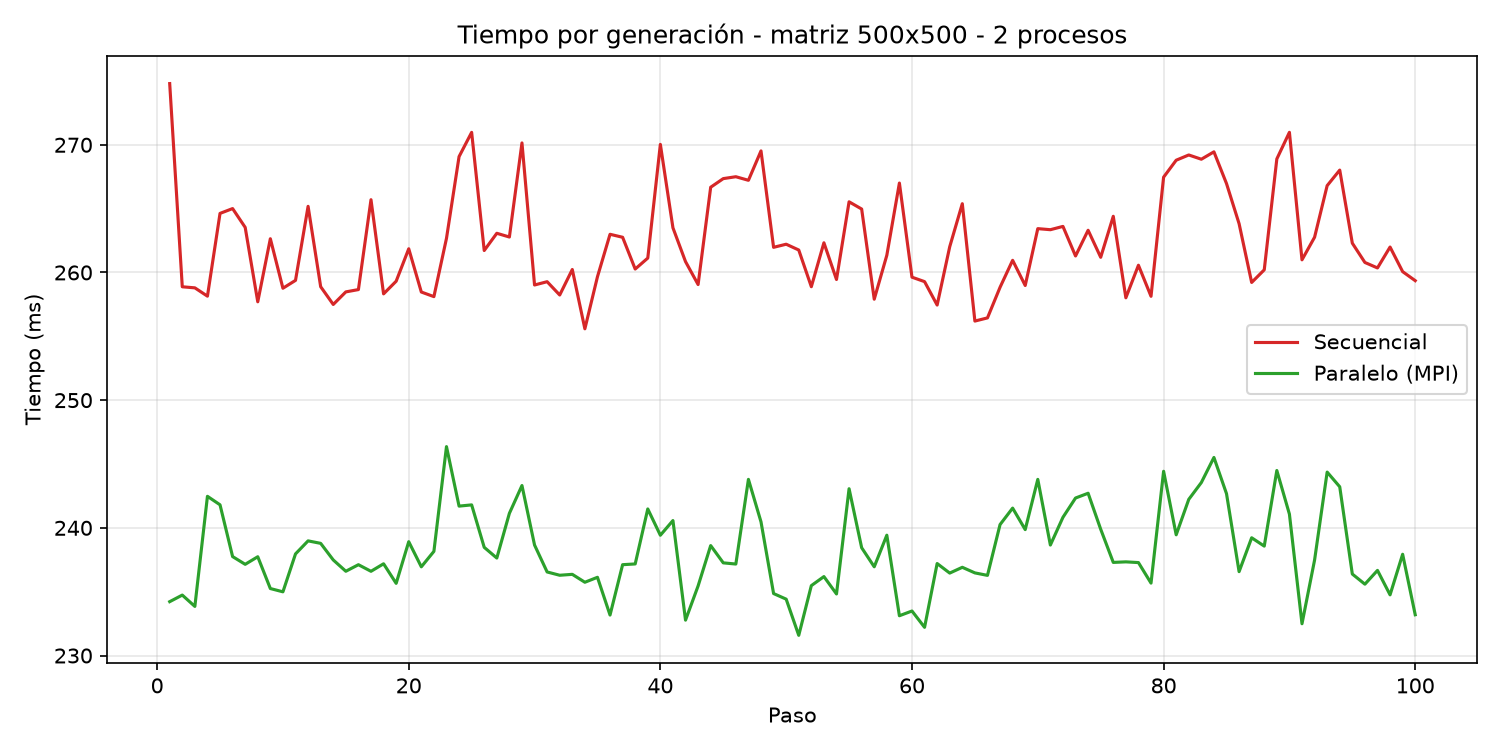
\includegraphics[width=\textwidth]{../resultados/tiempos_500x500_np2_20261014_145247_tiempo_por_paso.png}\\
        \small (a) 2 procesos
    \end{minipage}
    \hfill
    \begin{minipage}{0.49\textwidth}
        \centering
        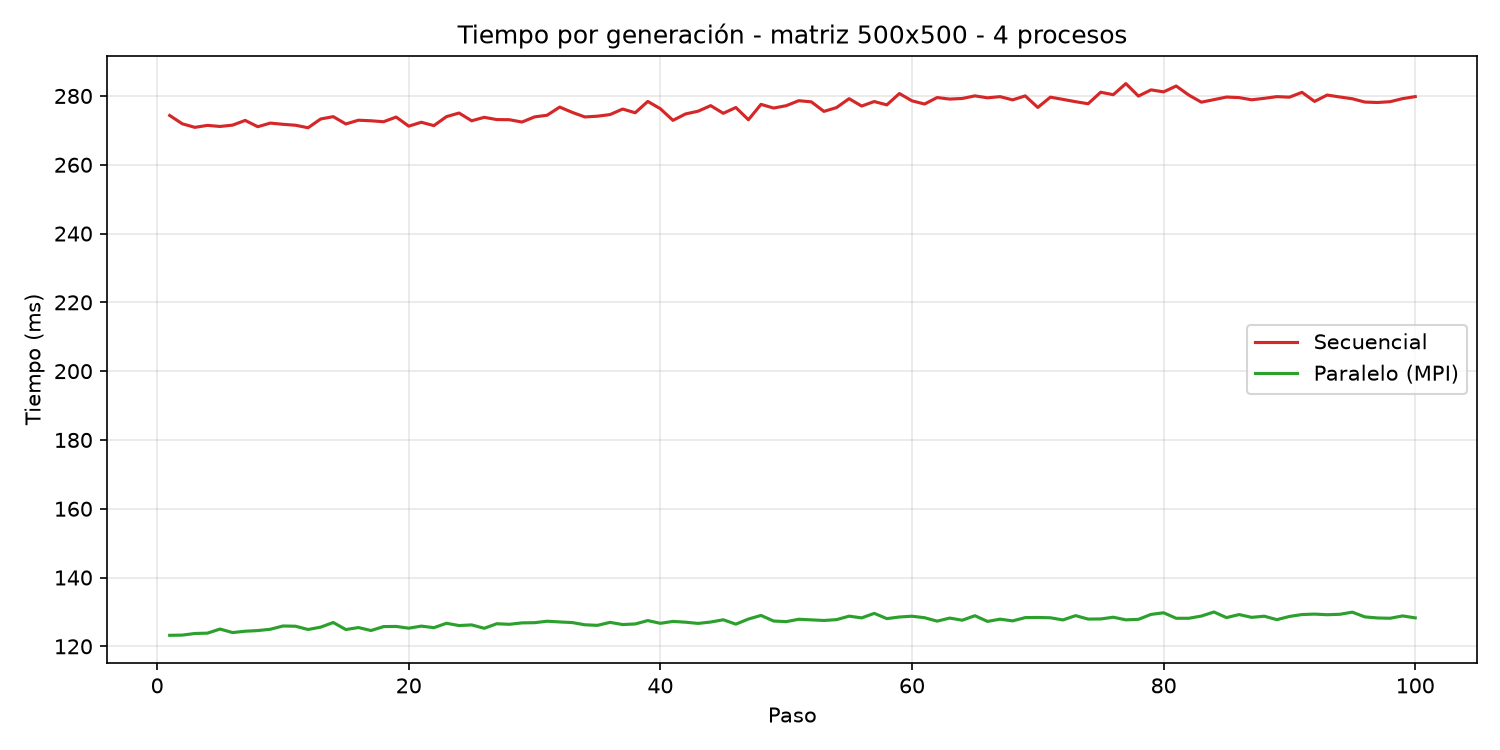
\includegraphics[width=\textwidth]{../resultados/tiempos_500x500_np4_20261014_145444_tiempo_por_paso.png}\\
        \small (b) 4 procesos
    \end{minipage}

    \vspace{0.4cm}

    \begin{minipage}{0.49\textwidth}
        \centering
        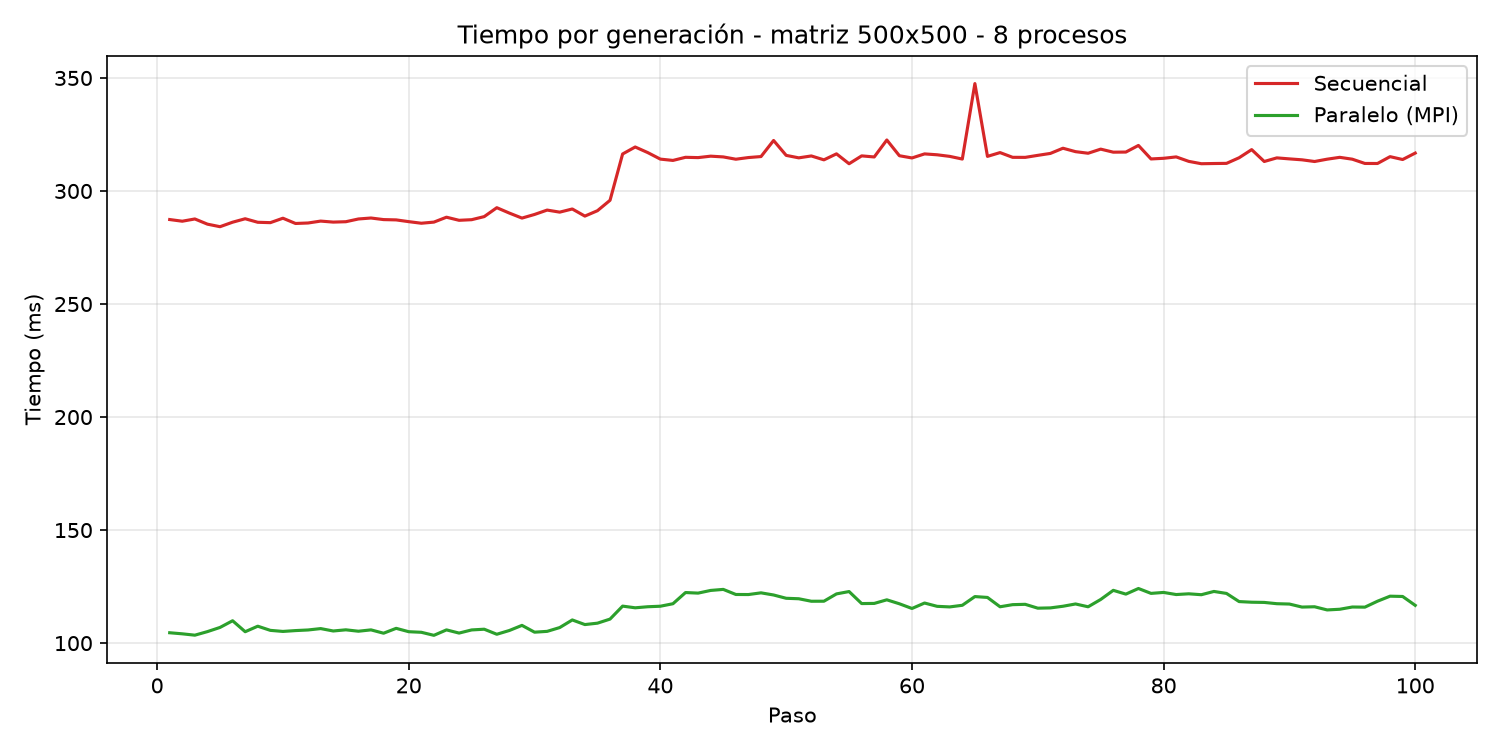
\includegraphics[width=\textwidth]{../resultados/tiempos_500x500_np8_20261014_145538_tiempo_por_paso.png}\\
        \small (c) 8 procesos
    \end{minipage}
    \hfill
    \begin{minipage}{0.49\textwidth}
        \centering
        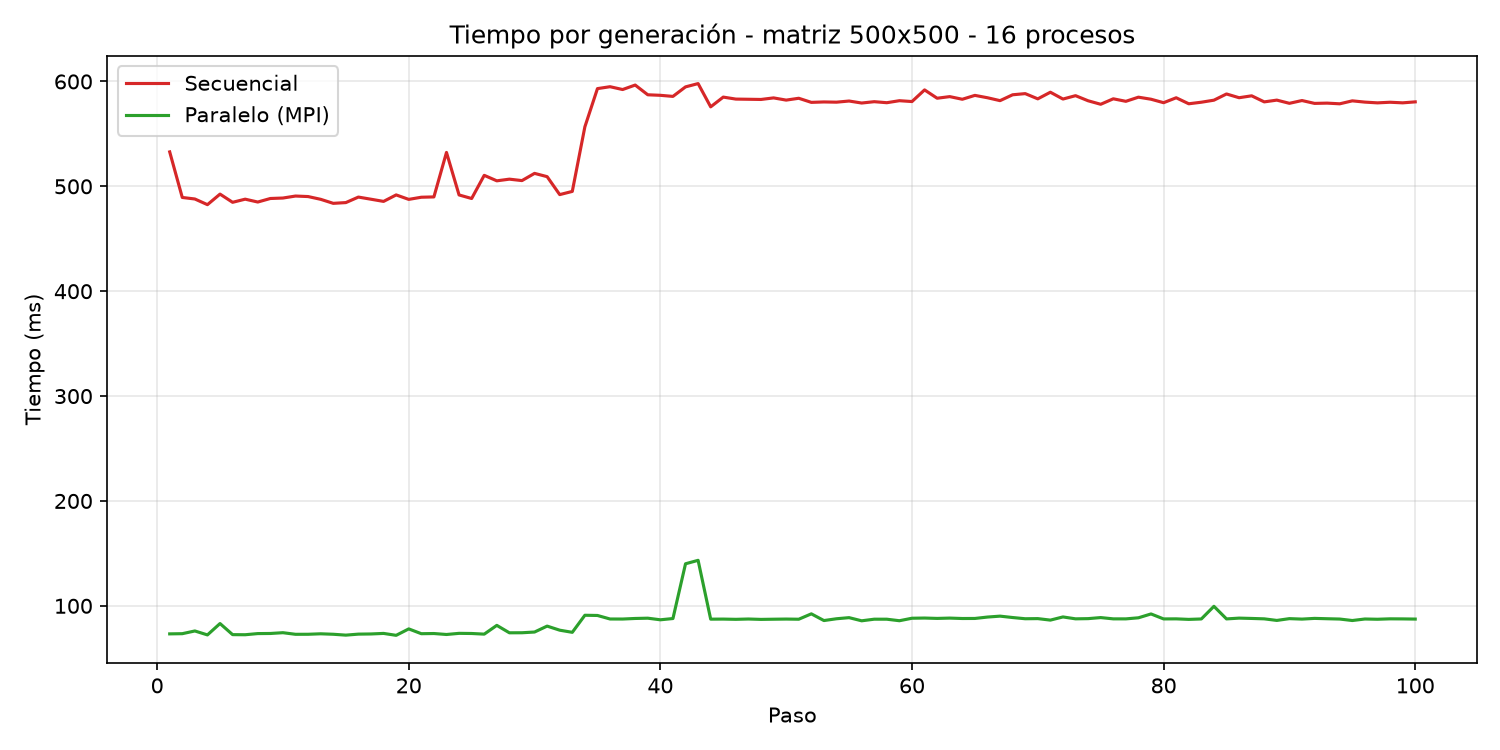
\includegraphics[width=\textwidth]{../resultados/tiempos_500x500_np16_20261014_145744_tiempo_por_paso.png}\\
        \small (d) 16 procesos
    \end{minipage}
    \caption{Tiempo por generación, secuencial vs. paralelo, tablero de $500 \times 500$.}
    \label{fig:procesos}
\end{figure}

\subsection{Variación del tamaño del tablero}
La tabla \ref{tab:tamanos} resume las pruebas con 4 procesos fijos. La fila de $500 \times 500$ corresponde a la misma prueba de la tabla \ref{tab:procesos}.

\begin{table}[H]
    \centering
    \begin{tabular}{|c|c|c|c|c|}
        \hline
        \textbf{Tablero} & \textbf{Secuencial (ms)} & \textbf{Paralelo (ms)} & \textbf{Speedup} & \textbf{Eficiencia} \\
        \hline
        $25 \times 25$     & $0.685 \pm 0.143$     & $0.495 \pm 0.148$    & $1.38$ & $0.35$ \\
        $50 \times 50$     & $2.631 \pm 0.262$     & $1.365 \pm 0.145$    & $1.93$ & $0.48$ \\
        $100 \times 100$   & $10.217 \pm 0.532$    & $4.936 \pm 0.183$    & $2.07$ & $0.52$ \\
        $500 \times 500$   & $276.500 \pm 3.275$   & $127.233 \pm 1.571$  & $2.17$ & $0.54$ \\
        $1000 \times 1000$ & $1203.675 \pm 20.344$ & $523.528 \pm 15.226$ & $2.30$ & $0.57$ \\
        \hline
    \end{tabular}
    \caption{Tiempo promedio por generación con 4 procesos, 100 generaciones.}
    \label{tab:tamanos}
\end{table}

\begin{figure}[H]
    \centering
    \begin{minipage}{0.49\textwidth}
        \centering
        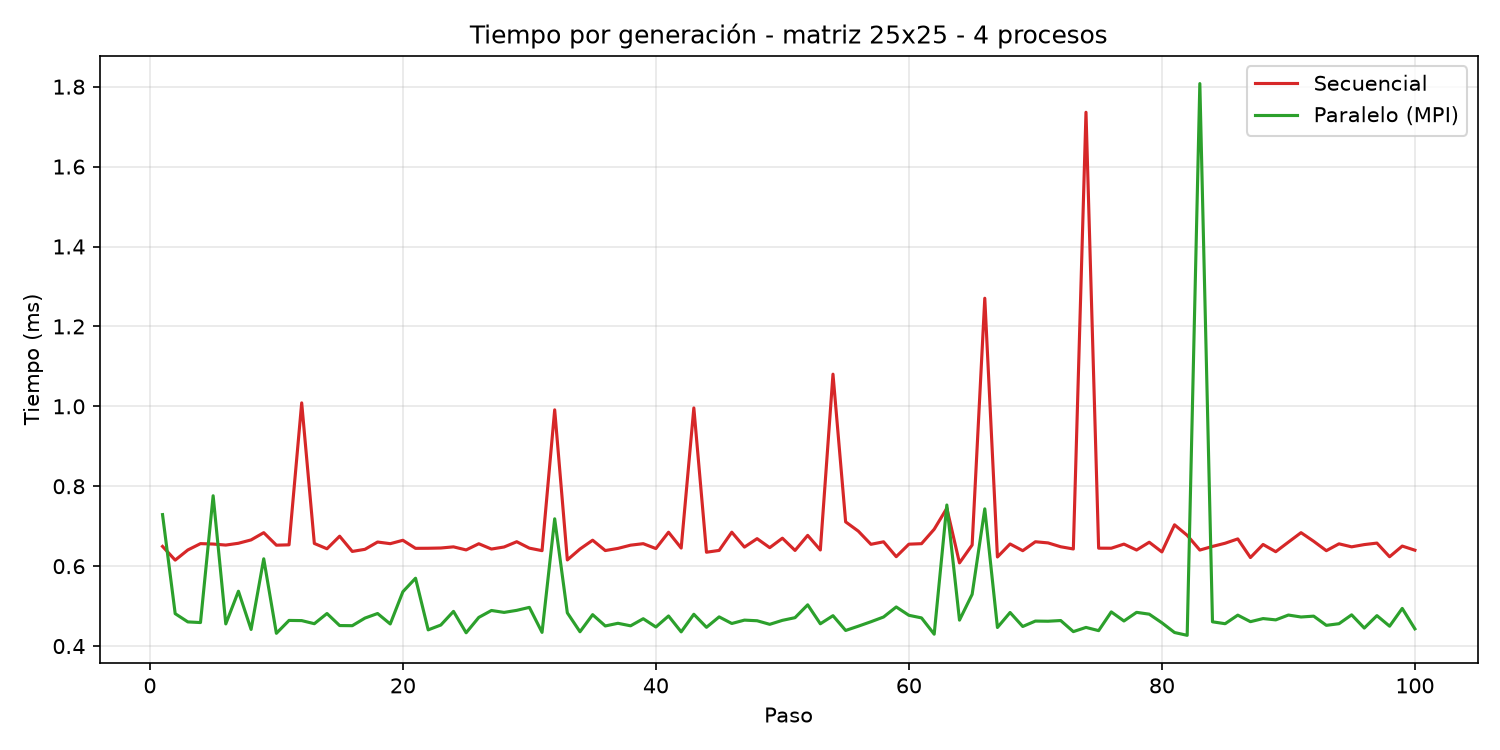
\includegraphics[width=\textwidth]{../resultados/tiempos_25x25_np4_20261013_002819_tiempo_por_paso.png}\\
        \small (a) $25 \times 25$
    \end{minipage}
    \hfill
    \begin{minipage}{0.49\textwidth}
        \centering
        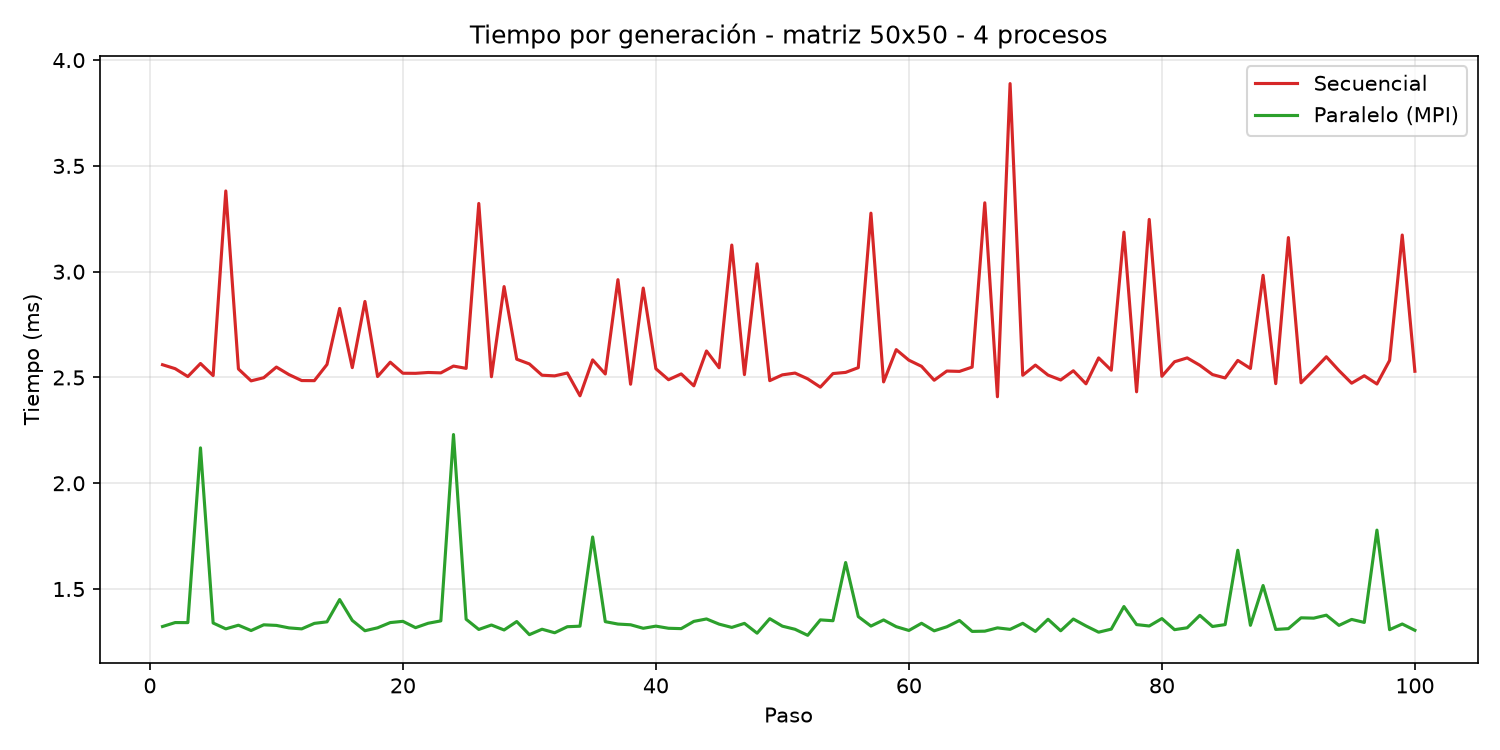
\includegraphics[width=\textwidth]{../resultados/tiempos_50x50_np4_20261013_003434_tiempo_por_paso.png}\\
        \small (b) $50 \times 50$
    \end{minipage}

    \vspace{0.4cm}

    \begin{minipage}{0.49\textwidth}
        \centering
        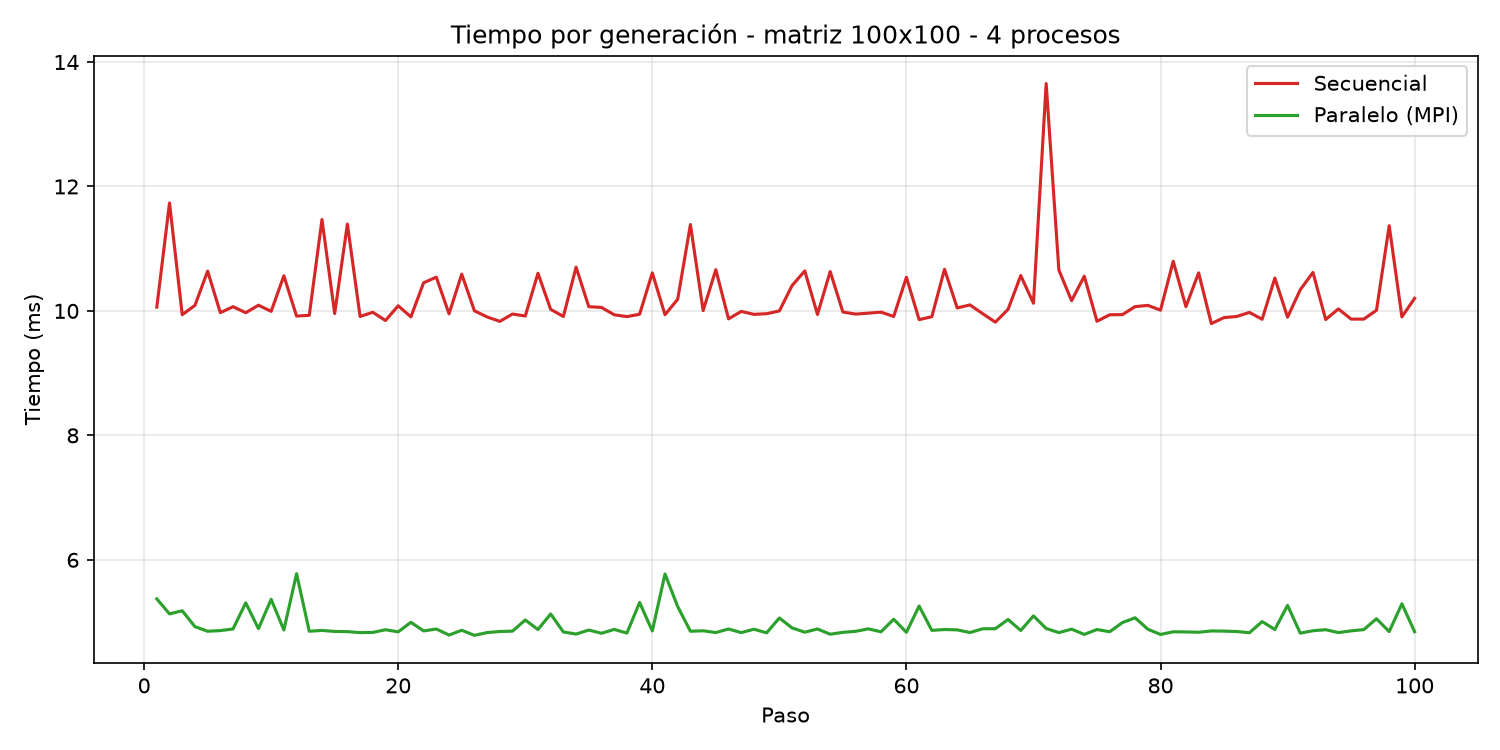
\includegraphics[width=\textwidth]{../resultados/tiempos_100x100_np4_20261013_003716_tiempo_por_paso.png}\\
        \small (c) $100 \times 100$
    \end{minipage}
    \hfill
    \begin{minipage}{0.49\textwidth}
        \centering
        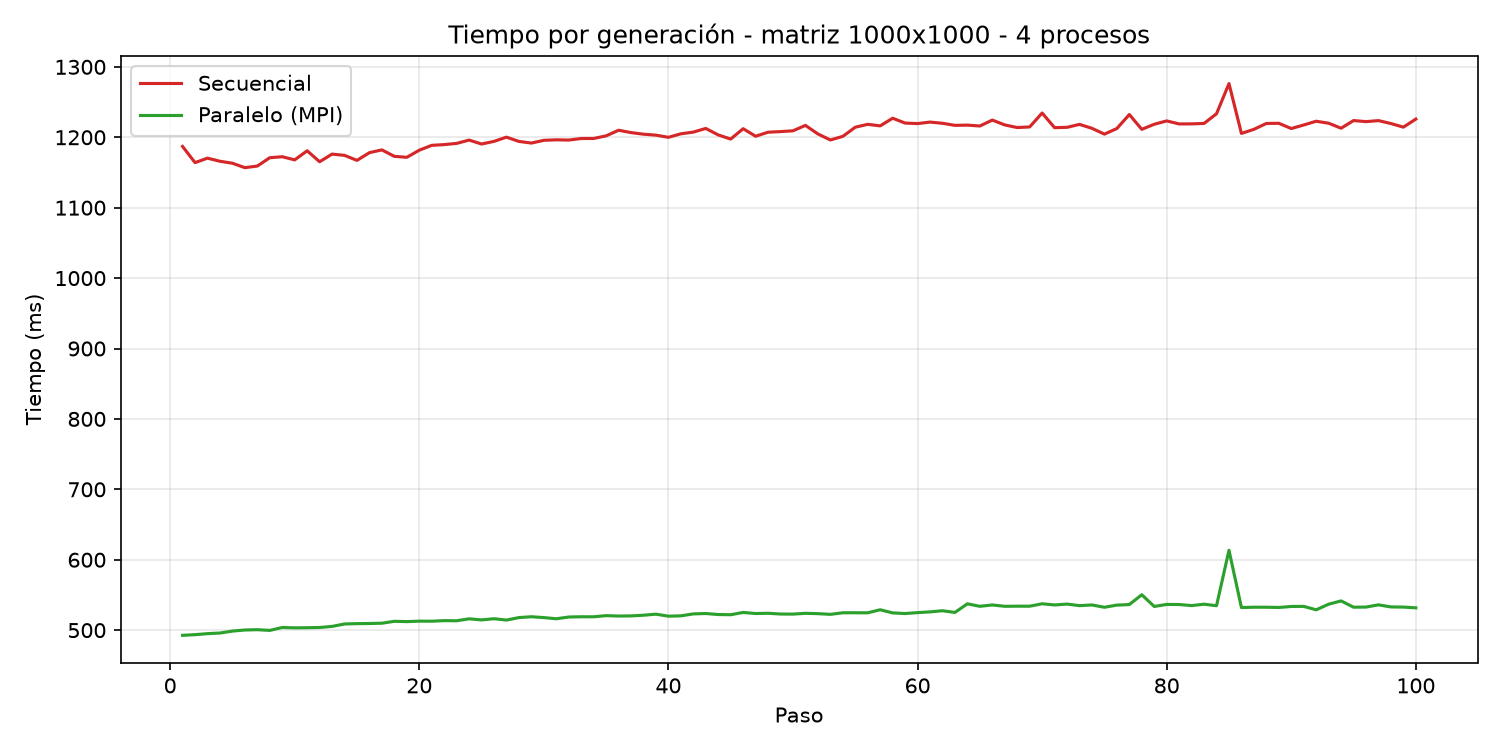
\includegraphics[width=\textwidth]{../resultados/tiempos_1000x1000_np4_20261013_004539_tiempo_por_paso.png}\\
        \small (d) $1000 \times 1000$
    \end{minipage}
    \caption{Tiempo por generación, secuencial vs. paralelo, con 4 procesos. La prueba de $500 \times 500$ con 4 procesos corresponde a la figura \ref{fig:procesos}(b).}
    \label{fig:tamanos}
\end{figure}

\section{Análisis}

\subsection{Efecto del número de procesos}
En el tablero de $500 \times 500$ el tiempo paralelo por generación disminuye de forma monótona al aumentar el número de procesos: pasa de $238.194$ ms con 2 procesos a $84.616$ ms con 16, es decir, una reducción de $2.81$ veces. Sin embargo, la ganancia entre configuraciones no es uniforme: al pasar de 2 a 4 procesos el tiempo se reduce $1.87$ veces, de 4 a 8 apenas $1.11$ veces y de 8 a 16 se reduce $1.35$ veces.\\

Un aspecto importante es que el tiempo del motor \textbf{secuencial} también cambia entre pruebas, aunque se ejecuta exactamente el mismo código sobre un tablero del mismo tamaño: $262.471$ ms con 2 procesos, $276.500$ ms con 4, $305.841$ ms con 8 y $554.153$ ms con 16. La explicación más probable es que el motor secuencial corre en el rango 0 mientras los demás procesos MPI siguen vivos en el mismo equipo, esperando el siguiente comando en \verb|comm.bcast|, por lo que comparten los recursos del procesador. Con 16 procesos se ocupan todos los hilos disponibles (y se superan los 12 núcleos físicos, de ahí la necesidad de \verb|--oversubscribe|), lo que coincide con el aumento más fuerte en esa prueba. En consecuencia, el \textit{speedup} de $6.55$ obtenido con 16 procesos está inflado por una línea base secuencial más lenta. Si se toma como referencia el tiempo secuencial de la prueba con menos procesos ($262.471$ ms), el \textit{speedup} con 4, 8 y 16 procesos sería de $2.06$, $2.30$ y $3.10$ respectivamente.\\

En las gráficas de 8 y 16 procesos (figura \ref{fig:procesos}(c) y (d)) se observa además un salto de nivel alrededor de la generación 35 que afecta al mismo tiempo a ambos motores, lo cual indica un factor del sistema durante la ejecución y no un cambio en el trabajo realizado por el algoritmo. Con 16 procesos también aparece un pico aislado en el tiempo paralelo cerca de la generación 42 (máximo de $143.388$ ms), que eleva su desviación estándar.\\

Por otro lado, con 2 procesos el \textit{speedup} es apenas de $1.10$, lejos del ideal de $2$. Si cada proceso procesa la mitad del tablero, el tiempo esperado sería cercano a $131$ ms, pero se midieron $238.194$ ms. Esto indica que el costo de procesar cada celda en el motor paralelo es mayor que en el secuencial. Al revisar el código, el motor secuencial recorre listas de Python, mientras que el motor paralelo recorre arreglos de NumPy accediendo elemento por elemento dentro de ciclos \verb|for| de Python (\verb|padded_grid[nr][nc]|), lo cual es más costoso que el acceso a listas. A esto se suma el costo de construir la vista local con \verb|np.vstack| y la comunicación de cada generación.

\subsection{Efecto del tamaño del tablero}
Con 4 procesos fijos el \textit{speedup} crece con el tamaño del tablero: $1.38$ en $25 \times 25$, $1.93$ en $50 \times 50$, $2.07$ en $100 \times 100$, $2.17$ en $500 \times 500$ y $2.30$ en $1000 \times 1000$. Lo mismo ocurre con la eficiencia, que pasa de $0.35$ a $0.57$.\\

Esto se explica por la relación entre cómputo y comunicación. En cada generación el trabajo de cálculo de cada proceso crece con el número de celdas de su franja ($\frac{filas \times columnas}{p}$), mientras que el intercambio de filas fantasma solo envía una fila completa a cada vecino, y el \textit{broadcast} del comando tiene un costo fijo. Por ello, en tableros pequeños el costo de comunicación y sincronización pesa más en proporción al cálculo. En el tablero de $25 \times 25$ los tiempos son menores a $1$ ms y la gráfica (figura \ref{fig:tamanos}(a)) muestra picos aislados en ambos motores, con un máximo paralelo de $1.808$ ms, por lo que en esta escala la variabilidad del sistema es comparable al tiempo mismo de cómputo.\\

En tableros grandes el comportamiento es mucho más estable: en $500 \times 500$ la desviación estándar paralela es de $1.571$ ms frente a un promedio de $127.233$ ms. Además, el tiempo crece de forma aproximadamente proporcional al número de celdas: al pasar de $500 \times 500$ a $1000 \times 1000$ (4 veces más celdas) el tiempo secuencial aumenta $4.35$ veces y el paralelo $4.11$ veces. En términos acumulados, las 100 generaciones del tablero de $1000 \times 1000$ tomaron $120.37$ s en el motor secuencial y $52.35$ s en el motor paralelo.\\

Aun en el tablero más grande, el \textit{speedup} con 4 procesos ($2.30$) no se acerca al ideal de $4$, lo cual es consistente con el mayor costo por celda del motor paralelo descrito en la sección anterior.

\subsection{Ventajas}
\begin{itemize}
    \item \textbf{Reducción real del tiempo por generación:} en todas las pruebas analizadas el motor paralelo fue más rápido que el secuencial, desde $1.10$ veces con 2 procesos hasta $6.55$ veces con 16 procesos en el tablero de $500 \times 500$.
    \item \textbf{Paralelismo real en Python:} al usar procesos con su propio intérprete en lugar de hilos, se evita la restricción del GIL y el cálculo de cada franja del tablero ocurre de forma simultánea en distintos núcleos.
    \item \textbf{Comunicación reducida:} la descomposición por dominio en franjas horizontales hace que cada proceso solo necesite intercambiar una fila con cada vecino por generación, por lo que la comunicación es pequeña frente al cálculo en tableros grandes.
    \item \textbf{Mejora con el tamaño del problema:} el \textit{speedup} y la eficiencia aumentan al crecer el tablero, que es justamente el escenario donde el motor secuencial se vuelve más lento.
    \item \textbf{Reparto de carga equilibrado:} las filas sobrantes de la división se reparten entre los primeros procesos, por lo que la diferencia de carga entre procesos es de máximo una fila.
    \item \textbf{Escalabilidad a memoria distribuida:} al estar basado en MPI, el mismo código podría ejecutarse en varios equipos o en un clúster sin cambiar el modelo de programación.
\end{itemize}

\subsection{Desventajas}
\begin{itemize}
    \item \textbf{Poco beneficio en tableros pequeños:} en el tablero de $25 \times 25$ el \textit{speedup} fue de $1.38$ con una eficiencia de $0.35$, ya que el costo de comunicación y sincronización es comparable al tiempo de cálculo.
    \item \textbf{Eficiencia lejana al ideal:} ninguna prueba superó una eficiencia de $0.57$, y con 2 procesos el \textit{speedup} fue de solo $1.10$, debido al mayor costo por celda del cálculo con arreglos de NumPy accedidos elemento por elemento.
    \item \textbf{Rendimientos decrecientes al aumentar procesos:} pasar de 4 a 8 procesos solo redujo el tiempo paralelo de $127.233$ ms a $114.247$ ms, y para usar 16 procesos fue necesario sobresuscribir los núcleos físicos del equipo.
    \item \textbf{Competencia por recursos:} los procesos MPI comparten el mismo equipo, lo que hizo que incluso el motor secuencial se volviera más lento al aumentar el número de procesos, de $262.471$ ms a $554.153$ ms.
    \item \textbf{Recolección centralizada:} en cada generación el tablero completo se reúne en el rango 0 con \verb|Gatherv| para poder visualizarlo, lo que concentra la comunicación en un único proceso.
    \item \textbf{Mayor complejidad:} la implementación requiere el modelo SPMD, un protocolo de comandos entre procesos, el cálculo de desplazamientos para \verb|Scatterv| y \verb|Gatherv|, y ejecutarse a través de \verb|mpiexec|, lo que también dificulta la depuración frente a la versión secuencial.
    \item \textbf{Mayor consumo de memoria:} cada proceso mantiene su propia instancia del intérprete de Python.
\end{itemize}

\section{Conclusiones}
\begin{itemize}
    \item La implementación paralela con MPI redujo el tiempo por generación del juego de la vida en todas las configuraciones probadas, alcanzando un \textit{speedup} de $6.55$ con 16 procesos en un tablero de $500 \times 500$ y de $2.30$ con 4 procesos en un tablero de $1000 \times 1000$.
    \item El beneficio del paralelismo depende del tamaño del problema: con 4 procesos el \textit{speedup} pasó de $1.38$ en el tablero de $25 \times 25$ a $2.30$ en el de $1000 \times 1000$, ya que en tableros grandes el cálculo domina sobre la comunicación.
    \item Aumentar el número de procesos reduce el tiempo paralelo, pero con rendimientos decrecientes, y al superar los núcleos físicos del equipo los procesos compiten por los recursos. Esta competencia también afectó la medición del motor secuencial, por lo que los \textit{speedups} de las pruebas con más procesos deben interpretarse junto con la línea base secuencial de cada prueba.
    \item La eficiencia obtenida (máximo $0.57$) muestra que hay margen de mejora en el cálculo local de cada proceso, en particular reemplazando el acceso elemento por elemento a los arreglos de NumPy, ya que este hace que procesar cada celda sea más costoso que en la versión secuencial.
    \item El uso de procesos mediante MPI, en lugar de hilos, permitió obtener paralelismo real en Python a pesar del GIL, y deja la solución preparada para ejecutarse en entornos de memoria distribuida.
\end{itemize}

\end{document}
